% Syslab Research Journal Template
% By Patrick White
% September 2019

% Do not edit this header
\documentclass[letterpaper,11pt]{article}
\usepackage{fullpage}
\usepackage{palatino}
\usepackage{courier}
\usepackage{graphicx}
\def\hrulefill{\leavevmode\leaders\hrule height 20pt\hfill\kern\z@}

% ------------- Edit these definitions ---------------------
\def\name{Bryan Lu}
\def\journalnum{7}
\def\daterange{10/14/19-10/28/19} % starts on Monday
\def\period{2}
% ------------------ END ---------------------------------
% Do not edit this
\begin{document}
	\thispagestyle{empty}
	\begin{flushright}
		{\Large Journal Report \journalnum} \\
		\daterange\\
		\name \\
		Computer Systems Research Lab \\
		Period \period, White
		\end{flushright}
	\hrule height 1pt

% ------ SECTION DAILY LOG -------------------------------------
\vspace{-0.8em}
\section*{Daily Log}
%Detail for each day about what you research, coded, debug, designed, created, etc. Informal style is OK.
\vspace{-0.8em}

\subsection*{Tuesday, October 15}
\vspace{-0.6em}
I completed \texttt{lexicon.txt}, which now holds all the words I'm looking for in every problem along with the objects and relations associated with them. 
\vspace{-1.3em}
\subsection*{Thursday, October 17}
\vspace{-0.6em}
I reconfigured detection code to accomodate double-word objects, and to detect any word in \texttt{lexicon.txt}.
%% relations -> turn them into names of actual functions, determine return type for them, whether they are unary/binary, explicit/implicit variable, word distance of objects, 
\vspace{-1.3em}
\subsection*{Monday, October 21}
\vspace{-0.6em}
I used the \texttt{nltk} library to get part-of-speech tags for every word, which will be used later.
\vspace{-1.3em}
\subsection*{Tuesday, October 22}
\vspace{-0.6em}
I calculated an index of every detected word or phrase in the sentence (treated as a list), which will give us sentence distancse easily when needed later. 
\vspace{-1.3em}
\subsection*{Thursday, October 24}
\vspace{-0.6em}
I created \texttt{finalrelations.txt}, which identifies the type of inputs, return type, and number of arguments each relation needs in each identified relation in the sentence. 
% ------ SECTION TIMELINE -------------------------------------
%\newpage
%\vspace{-1.7em}
\vspace{-1.7em}
\section*{Timeline}
\begin{tabular}{|p{1in}|p{2.5in}|p{2.5in}|}
	\hline
\textbf{Date} & \textbf{Goal} & \textbf{Met}\\ \hline 
	\hline 
10/7 & Create a logical language to give more structure and properties to the objects and relations detected in the problem.  & Not quite the goal I needed to meet, but I figured out the path I need to take going forward and started creating the dictionary I needed to have for my problem. \\
	\hline 
10/14 & Finalize the object identification associated with \texttt{lexicon.txt}, and figure out how to extract the necessary data to pass to the log-linear classifier. & I completed this successfully, but without much time this week I only started to come up with some ideas as to how to extract the necessary data. \\
	\hline 
10/21 & Complete the extraction of all the necessary features of the sentences needed as input data. & Almost -- I have found all of the necessary features except for ``dependency tree distance.'' \\
	\hline 
10/28 & Begin writing code to create a log-linear classifier using \texttt{scikit}, and finalize the inputs needed for the algorithm. & N/A  \\
	\hline
11/4 & Create the log-linear classifier/learning algorithm and the training data, and begin testing. & N/A \\
	\hline
\end{tabular}


% ------ SECTION REFLECTION  ---------------------------------
\section*{Reflection}
%In narrative style, talk about your work this week. Successes, failures, changes to timeline, goals. This should also include concrete data, e.g. snippets of code, screenshots, output, analysis, graphs, etc.

The past two weeks have seen me finish almost all of the necessary setup needed for the first major stage of my project. I can. Here is a snippet of the completed \texttt{relations.txt} (for now): 
\begin{center}
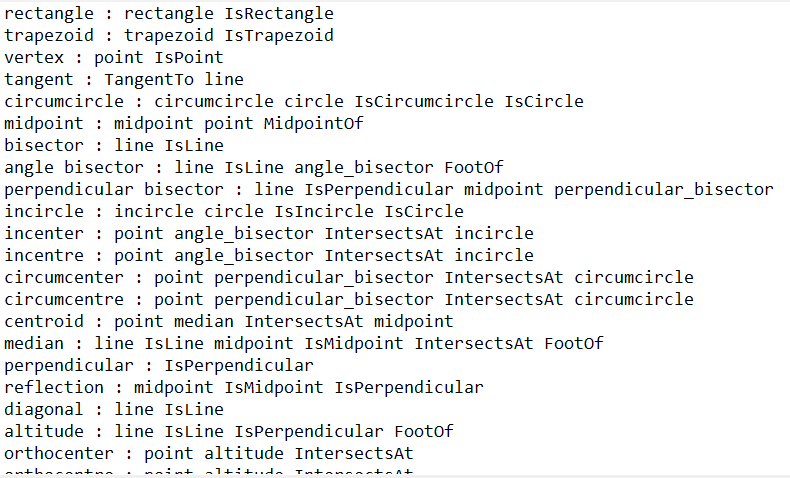
\includegraphics[scale=0.5]{lexiconfinish.png}
\end{center}
Note the two-word phrases, which I had to adapt my code to handle, and the mixture of objects and relations with many of the words. It's easy to add to the list of objects and relations associated with each word I want to detect, and it's fairly straightforward to add more words/symbols I want to detect in the sentence to the text file. I think my code can handle it as long as the word/phrase is at most two words. This versatility is something I will probably want later for ease of modification. 

One challenge I will likely face in the coming weeks is the fact that I have to train two (and possibly more!) different log-linear classifiers to identify whether or not a given relation with inputs is valid. Granted, given the properties of the relations, which I have articulated in a separate file (\texttt{finalrelations.txt}), most of the relations are one-argument functions:
\begin{center}
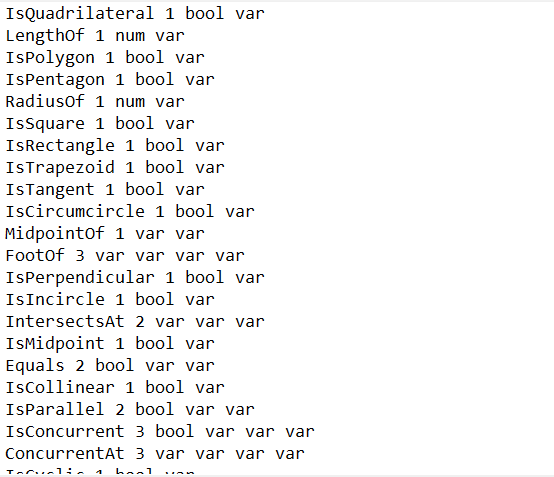
\includegraphics[scale=0.5]{relations.png}
\end{center}
This means it's plausible for me to handle these separately, but I'm not sure how reliable that will be. 

Regardless, I will soon be on my way to create the main machine-learning part of my model, and here is where the test cases and problems I have gathered in the past will come in handy. I have found a website where someone has gathered a lot of problems in one place, so I might consider taking a bit of time on a weekend to scrape it to add to my data set. Currently, I am techinically still on schedule, as next week should be week 2 of 4 of writing and training the log-linear classifier, so I'm optimistic about finishing this important phase of the project on time. 

\end{document}

